% Chapter 4

% NOTE: 1. REPLACE THE MODEL AND DP BY SENSYS PAPER, RESIMULATE THE RESULTS FOR CPH AND ADD THE RESULT OF DP 

\chapter{Error Correction Codes in optical interconnects -- Energy efficiency channel} % Write in your own chapter title
\label{SmartSense}
%\addtotoc{State of the Arts}
\lhead{\emph{SmartSense: Sensor-Aided NILM}} % Write in your own chapter title to set the page header

\section{The transmitted laser power and communication loss modeling}\label{model}
\subsection{Point-to-point optical interconnect}
In NILM, the disaggregation algorithms always try to extract the features from the overall electrical load signal to identify the devices. However, how can we discern the devices with the same power characteristics? For example~\cite{Laughman03PEM}, if the algorithms use the features related to the average power consumption such as power level, length of steady state, step-change, etc., to discriminate the devices, it can lead to a false detection when  separating an incandescent light bulb and a desktop computer, which consume the same power of 150W.
\subsection{Model of loss}

%---------------------------------
\begin{figure}[!hbt]
\begin{center}
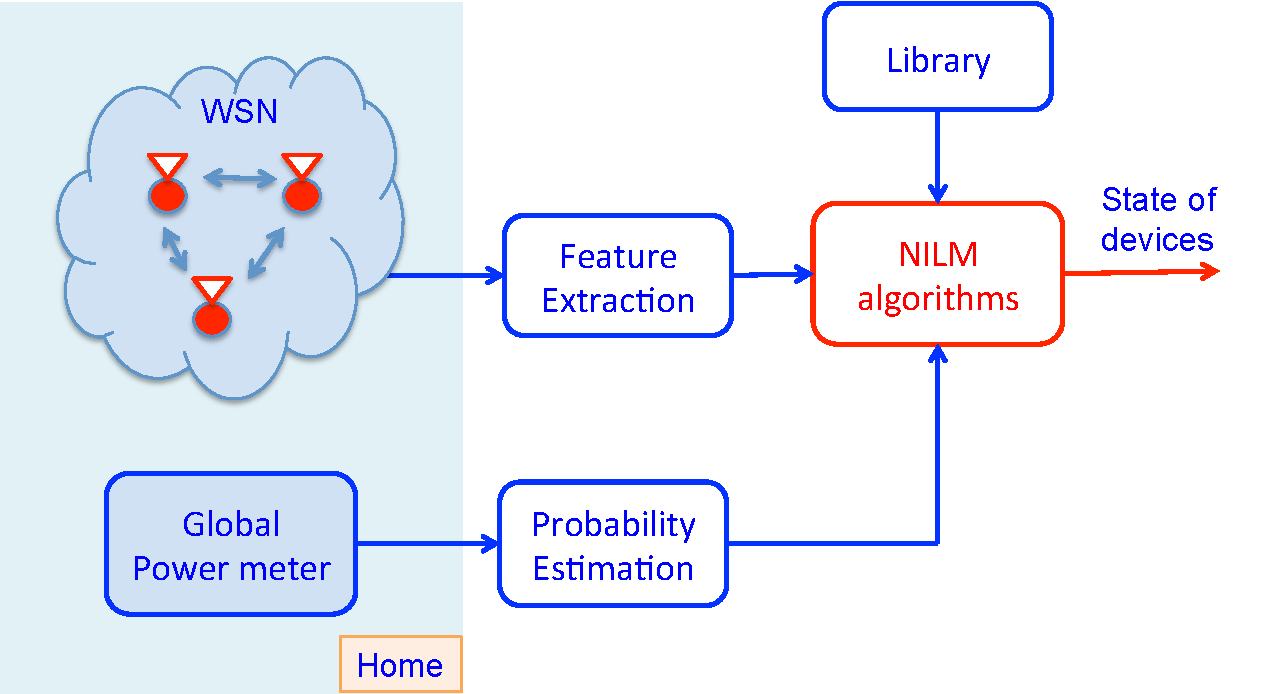
\includegraphics[width=1\textwidth]{./chapters/chapter4/images/SSmodel.pdf}
\caption{SmartSense system model: an NILM system combining with a sensor network providing the operating probability of some specific devices.}
\label{fig:S1}
\end{center}
\end{figure}

To overcome this restriction and improve the performance of the detection algorithms, we propose to use the operating probability of each device as an additional feature. A low-cost and low-power WSN is proposed to be deployed in homes and buildings to monitor the operation of some specific devices. A system combining NILM with such a WSN, called SmartSense, is shown in Figure~\ref{fig:S1}. However, different from ViridiScope~\cite{Kim09Ubicomp} which is fully intrusive, our approach only monitors a subset of all devices, which makes it less intrusive. On the other hand, the purpose of the WSN is not to directly provide the state of devices but to estimate their state probability to improve the performance of NILM algorithms. Depending on the type of monitored devices, the corresponding sensors are deployed.
For example, the operation of light-emitting devices such as screens, televisions, lamps can be detected by using the light intensity sensors, while the motor-based devices such as washing machine, fridge can be identified with a vibration sensor. Besides, other types of sensors can also be used to monitor other electrical equipment such as microphones, magnetometers, etc. A local algorithm in the WSN is then constructed to transform the detection of sensors to the probability of the corresponding devices. The probability estimation is executed based on the performance evaluation metrics including \textit{precision} and \textit{negative predictive value}, calculated by
\begin{eqnarray}
pr &=& \frac{TP}{TP+FP}\\
npv &= &\frac{TN}{TN+FN},
\end{eqnarray}
where $pr$, $TP$, $FP$ and $FN$ are defined in Chapter~\ref{l1norm} on page~\pageref{eva-metrics}, while $npv$ and $TN$ denote the negative predictive value and the number of true negatives, respectively. A true negative is defined as a true detection of non-event. Therefore, the negative predictive value can be considered as the reliability of a detected non-event.
As a consequence, when a device is determined as running, the probability of on-state and off-state are equal to $pr$ and $(1-pr)$, respectively. In contrast, when not running, they correspond to $(1-npv)$ and $npv$. For other unmonitored devices, all states can occur with the same probability.
\subsection{BER and Laser Power Trade-Offs for uncoded optical interconnect}
To prove the efficiency of the operating probability in improving the performance of NILM, in this research, we propose two main approaches for the state detection. In the first approach, the minimization problem \eqref{eqL1} of NILM can be modeled as a Knapsack problem and solved by two proposed algorithms including Compositional Pareto-algebraic Heuristic (CPH) and Dynamic Programming (DP). Meanwhile, the second one applies the probability to two existing algorithms including edge detection~\cite{Hart92} and dynamic time warping~\cite{Liao14}. In the rest of this chapter, the word \textit{event} is used to denote an on-state in the CPH, DP and DTW algorithms and an edge in the ED one.






\section{Error Correction Codes for optical interconnects}\label{knapsack}
%%------------------ modification: add a part of one-state devices
Let consider again the $l1$-norm minimization problem \eqref{eqL1} of NILM:
\begin{eqnarray}\label{eqSS2}
& &\min_{\mathbf{s}}{E(\mathbf{s}) = \left|\sum_{i=1}^N{\sum_{j=1}^{m_i}{w_{ij}s_{ij}}}-x\right|} \\
\mbox{subject to}&&s_{ij}\in \{0,1\},  i=1,\ldots,N,j=1,\ldots,m_i \nonumber\\
& & \sum_{j=1}^{m_i}{s_{ij}}\in \{0,1\}, i=1,\ldots,N, \nonumber
\end{eqnarray}
where $E(\mathbf{s})$ can be interpreted as the absolute error between the measured aggregate power consumption and the total power demand of all operating devices. Solving Eq.~\eqref{eqSS2} is equivalent to find a vector $\mathbf{s}$ comprising all state indicators $s_{ij}$, $i=1,\ldots,N, j=1,\ldots,m_i$ of all devices, i.e., $\mathbf{s}=\{s_{11},\ldots,s_{1m_1},s_{21},\ldots,s_{2m_2},\ldots,s_{N1},\ldots,s_{Nm_N}\}$.
In Chapter \ref{l1norm}, this problem is solved by applying three proposed methods including least absolute error, state difference and state transition probability. However, in the SmartSense system, by using an additional parameter related to the operating probability, a new problem is formulated from \eqref{eqSS2} and two methods are proposed to solve it including CPH and DP. The on/off state probability of each device is estimated as mentioned in Section \ref{model}. Nevertheless, as the sensors can only detect if a device is on or off but cannot distinguish its different power states, the operating probability will then be equally divided to all states, i.e. $p_{ij} = p_i/m_i,j=1,\ldots,m_i$. Let consider the problem formulation in the case that each device has only two states, on or off, and in a general case in which each device has a finish number of power states.


\subsection{Problem formulation}
%%------------------ modification: add a part of one-state devices

\paragraph*{One-state devices}
Firstly, let consider the simplest case in which each device can only operate at a unique stable state with a corresponding power demand $w_i$. Denote $s_i$ as the state indicator of device $i$ and notation $^{(1)}$ for one-state using case, problem \eqref{eqSS2} becomes:
\begin{eqnarray}\label{eqSS3}
& &\min_{\mathbf{s}}{E^1(\mathbf{s})=\left |\sum_{i=1}^N{w_is_i}-x\right |}\\
\mbox{subject to } & &s_i\in \{0,1\}, i=1,\ldots ,N, \nonumber
\end{eqnarray}
where $\mathbf{s} = \{s_1,s_2,\ldots ,s_N\}$.
Assuming device $i$ is in on-state with probability of $p_i,0\leq p_i\leq 1$, the probability mass function is then:
\begin{equation}\label{eqSS4}
Pr(s_i) = p_i^{s_i}(1-p_i)^{(1-s_i)}.
\end{equation}
%
Because the operation of $N$ devices is assumed to be independent, the coincidence probability, the probability that all events happen simultaneously, is as follows:
\begin{eqnarray}\label{eqSS6}
Pr(\mathbf{s})& =& \prod_{i=1}^N{Pr(s_i)}\nonumber \\
&=&\prod_{i=1}^N{p_i^{s_i}(1-p_i)^{(1-s_i)}}.
\end{eqnarray}
To reduce the computational complexity, the log-linear form can be applied to transform the multiplication in~\eqref{eqSS6} to an addition, which gives:
\begin{eqnarray}\label{eqSS7}
L^1(\mathbf{s}) &=& -\log{(Pr\left(\mathbf{s})\right)} \nonumber \\
&=&-\log{\left( \prod_{i=1}^N{p_i^{s_i}(1-p_i)^{(1-s_i)}}\right)}\nonumber \\
&=& -\sum_{i=1}^N{\left(s_i\log{p_i}+(1-s_i)\log{(1-p_i)}\right)}.
\end{eqnarray}
Denote $L^1(s_i) = (1-s_i) l^1_{i0}+s_i l^1_{i1}$ with $l^1_{i0} = -\log{(1-p_i)}$ and $l^1_{i1} = -\log{p_i}$, Eq.~\eqref{eqSS7} can be written as
\begin{eqnarray}
L^1(\mathbf{s}) &=& \sum_{i=1}^N{L^1(s_i)}.
\end{eqnarray}
By this transformation, the increase of $Pr(\mathbf{s})$ corresponds to the decrease of $L^1(\mathbf{s})$. The problem is now to find a combination of operating devices not only giving the least absolute error $E^1(\mathbf{s})$ but also having the maximum probability, i.e. the minimum value of $L^1(\mathbf{s})$. Therefore, the problem~\eqref{eqSS3} is developed to a co-optimization problem as follows:
\begin{eqnarray}\label{eqSS8}
& &\min_{\mathbf{s}}{\left[P^1(\mathbf{s}) = E^1(\mathbf{s}) + \lambda \times L^1(\mathbf{s})\right]}\\
\mbox{subject to } & & \sum_{i=1}^N{w_is_i} \leq x+\epsilon \nonumber \\
& &s_i\in \{0,1\}, i=1,\ldots ,N, \nonumber
\end{eqnarray}
where $\lambda$ is a regularization parameter and empirically chosen, $\epsilon$ corresponds to the standard deviation of the aggregate power consumption. The problem~\eqref{eqSS8} is a kind of \textbf{0-1 Knapsack problem}, in which the aim is to fill the knapsack by selecting among various objects, each of which having a particular weight and giving a particular profit~\cite{Lagoudakis96the0-1}. The optimization problem is then to choose the objects in order to obtain the maximum profit while respecting the knapsack capacity.
%%------------------ end modification




%=======================================
\paragraph*{Multi-state devices}
Return to the general case where each device has a finite number of states, the following condition needs to be satisfied:
\begin{equation}
\sum_{j=1}^{m_i}{s_{ij}}\leq 1,s_{ij} \in \{0,1\}, i=1,\ldots,N,
\end{equation}
where $m_i$ is the number of states of device $i$.
Therefore, the operating probability of device $i$, denoted as $Pr(\mathbf{s}_i)$, $\mathbf{s}_i = \{s_{i1},s_{i2},\ldots,s_{im_i}\}$, is
\begin{eqnarray}\label{eqSS9}
Pr(\mathbf{s}_i) = p_{i0}^{\prod_{j=1}^{m_i}{(1-s_{ij})}}\times \prod_{k=1}^{m_i}{p_{ik}^{\prod_{j=1,j\neq k}^{m_i}{s_{ik}(1-s_{ij})}}},
\end{eqnarray}
where  $p_{i0} = p(s_{ij}=0, j=1,\ldots,m_i)$ is the probability of off-state of device $i$ and $p_{ik} = p(s_{ik}=1,s_{ij}=0,\forall j\neq k)$ is the probability of operating at state $k$. Intuitively, we have $\sum_{j=0}^{m_i}{p_{ij}}=1$. 
Transforming Eq.~\eqref{eqSS9} to log-linear form gives
\begin{eqnarray}\label{eqSS10}
L^M(\mathbf{s}_i) &=& -\log{Pr(\mathbf{s}_i)} \nonumber\\
&=& -\prod_{j=1}^{m_i}{(1-s_{ij})}\log{p_{i0}} \nonumber \\
&& - \sum_{k=1}^{m_i}{\left\{\prod_{j=1,j\neq k}^{m_i}{s_{ik}(1-s_{ij})}\log{p_{ik}}\right\}}.
%&=& \sum_{j=0}^{m_i}{l_{ij}}.
\end{eqnarray}
Denoting $l^M_{ik} = -\log{p_{ik}}, k=0,\ldots,m_i$, Eq.~\eqref{eqSS10} can be rewritten as
\begin{equation}
L^M(\mathbf{s}_i) = \prod_{j=1}^{m_i}{(1-s_{ij})l^M_{i0}}+\sum_{k=1}^{m_i}{\left\{\prod_{j=1,j\neq k}^{m_i}{s_{ik}(1-s_{ij})}l^M_{ik}\right\}}.
\end{equation}
Similarly to the case of one-state devices, the concincidence probability $Pr(\mathbf{s})$, $\mathbf{s} = \{\mathbf{s}_1,\ldots,\mathbf{s}_N\}$, and its respective log-linear form $L^M(\mathbf{s})$ can be formulated as
\begin{eqnarray}\label{eqSS11}
Pr(\mathbf{s}) &=& \prod_{i=1}^N{Pr(\mathbf{s}_i)}\\
L^M(\mathbf{s})& =& \sum_{i=1}^N{L^M(\mathbf{s}_i)}.
\end{eqnarray}

As a consequence, the co-optimization problem to minimize the least absolute error in problem~\eqref{eqSS2} and maximize the coincidence probability in Eq.~\eqref{eqSS11} is modified to
\begin{eqnarray}\label{eqSS12}
&&\min_{\mathbf{s}}{\left[P^M(\mathbf{s}) = E^M(\mathbf{s}) + \lambda \times L^M(\mathbf{s})\right]} \\
\mbox{subject to } &&\sum_{i=1}^N{\sum_{j=1}^{m_i}{w_{ij}s_{ij}}}\leq x+\epsilon \nonumber\\
&& \sum_{j=1}^{m_i}{s_{ij}} \leq 1, j=1,\ldots,N \nonumber\\
&&s_{ij}\in \{0,1\},  i=1,\ldots ,N,j=1,\ldots,m_i.\nonumber
\end{eqnarray}
Considering the state of devices as objects and the aggregate power consumption as the knapsack capacity, Eq.~\eqref{eqSS11} is equivalent to the Knapsack problem. The state detection is apparently similar to dividing the available objects into groups and selecting a maximum of one object from each group to fill the knapsack. Hence, the problem~\eqref{eqSS12} can be considered as a so-called \textbf{Multiple-Choice Knapsack (MCK)} problem~\cite{Bean88}.

In SmartSense, at each data point, an algorithm will be applied to solve the co-optimization problem to find the corresponding state of each device. To solve the Knapsack problem, the naive and straightforward approach is brute force, as introduced in Chapter~\ref{l1norm}. However, the exponential complexity makes it intractable with large number of devices. Besides, there are several other approaches such as branch and bound \cite{Martello1980276,DYER1984231,Lukata1997}, genetic algorithm \cite{Anagun2006,Singh07,Fukunaga08,Shen11}, dynamic programming (DP)~\cite{Toth79,Bean88}, compositional Pareto-algebraic heuristic (CPH) \cite{Shojaei13,Shojaei5227146,Geilen07,Geilen05,Geilen07acm,Hifi04,Yukish2004}, or combining DP with branch and bound~\cite{Martello99}.

In this study, we focus on CPH and DP, two most effective approaches in Knapsack problem, to apply in the context of SmartSense. These algorithms have some driving parameters allowing to reduce the computational complexity.


\subsection{Error Correction Code implementations -- Case study}\label{sec:algo}
\subsubsection{Extended Hamming codes }\label{CPH}
%---------------------------------

The CPH algorithm is based on a recursive relation  and illustrated by an example in Figure~\ref{fig:SS2}. Figure~\ref{fig:SS2}(a) presents a set of three devices with different operation states. Each state consumes a stable power with a corresponding probability. Assuming at time instant $t$, the aggregate power consumption $x$ is equal to 150~W. With the standard deviation $\epsilon$ of 5~W, the total power demand of any set of operating devices cannot exceed the bound $R=x +\epsilon = 155$~W. Figure~\ref{fig:SS2}(b) shows how the CPH algorithm operates. In the first step, each device is represented as a set of \textit{tuples}, each corresponding to a state. For example, device $D_1$ comprises three tuples: $(0, 23.03,173.03)$, $(50,2.23,102.23)$, $(150,23.03,23.03)$. The first element $d_1$ of each tuple represents the power demand, the second one $d_2$ contains the product of the operating probability in log-linear form and the regularization parameter $\lambda$, equal to 10 in this example, and the third one $d_3$ is calculated from two first elements $d_1$ and $d_2$ as follows:
\begin{eqnarray}
d_1 &=& w\\
d_2 &=& -\lambda \times \log{p}\\
d_3 &=& \left|x-d_1\right|+d_2. \label{eqCPH1}
\end{eqnarray}
\begin{figure}[h]
%\centering
\begin{minipage}[b]{1\linewidth}
  \centering
  \centerline{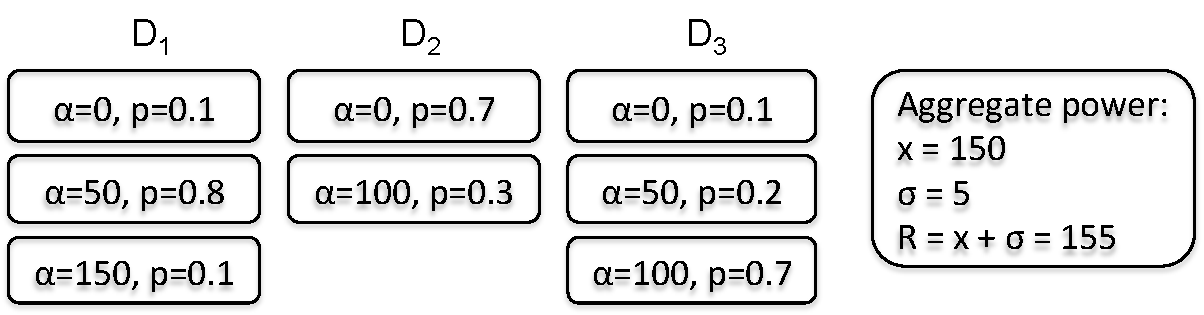
\includegraphics[width=0.8\textwidth]{./chapters/chapter4/images/cph1}}
%  \vspace{2.0cm}
  \centerline{(a)}\medskip
\end{minipage}
\begin{minipage}[b]{1\linewidth}
  \centering
  \centerline{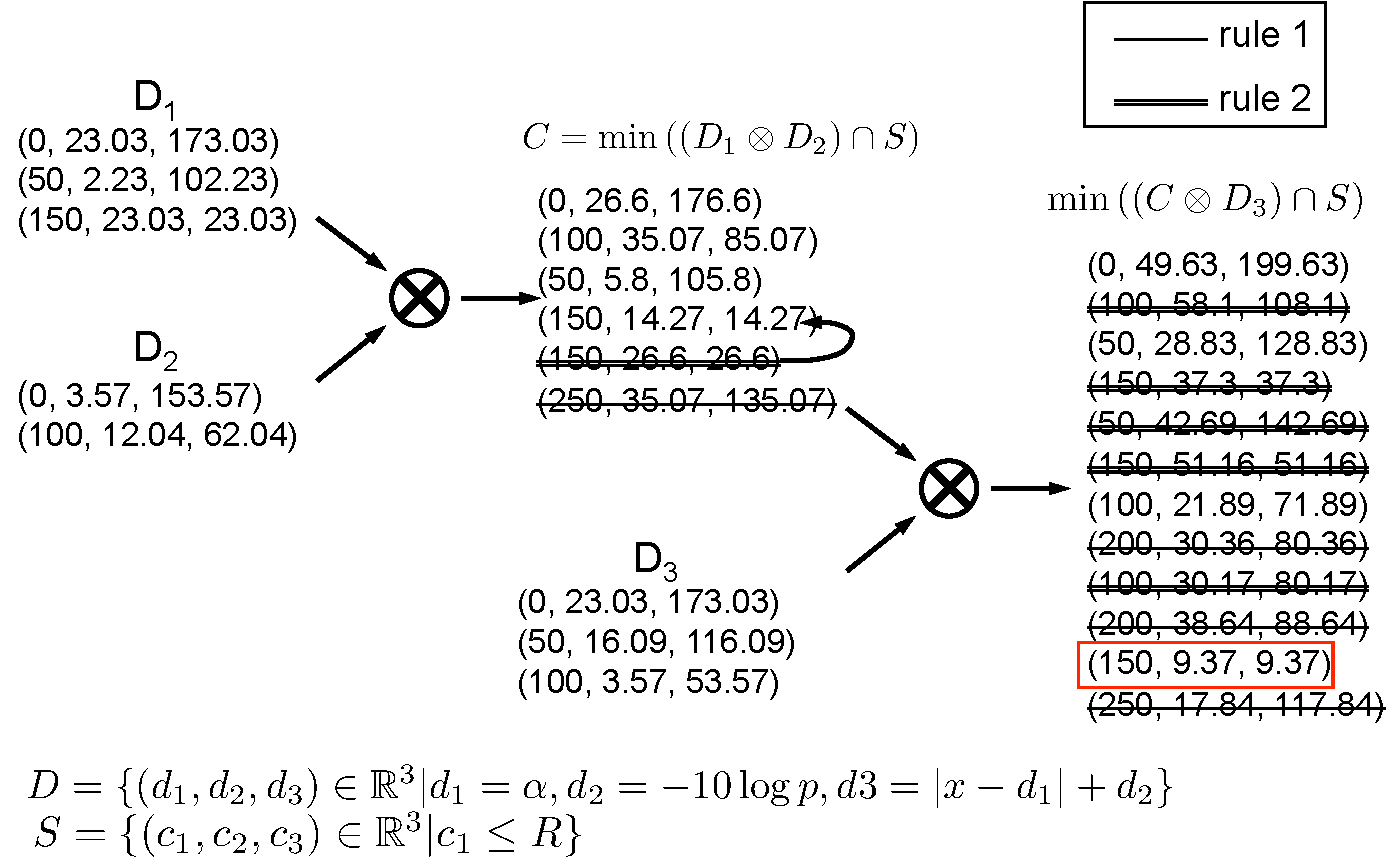
\includegraphics[width=0.9\textwidth]{./chapters/chapter4/images/cph2}}
%  \vspace{2.0cm}
  \centerline{(b)}\medskip
\end{minipage}
%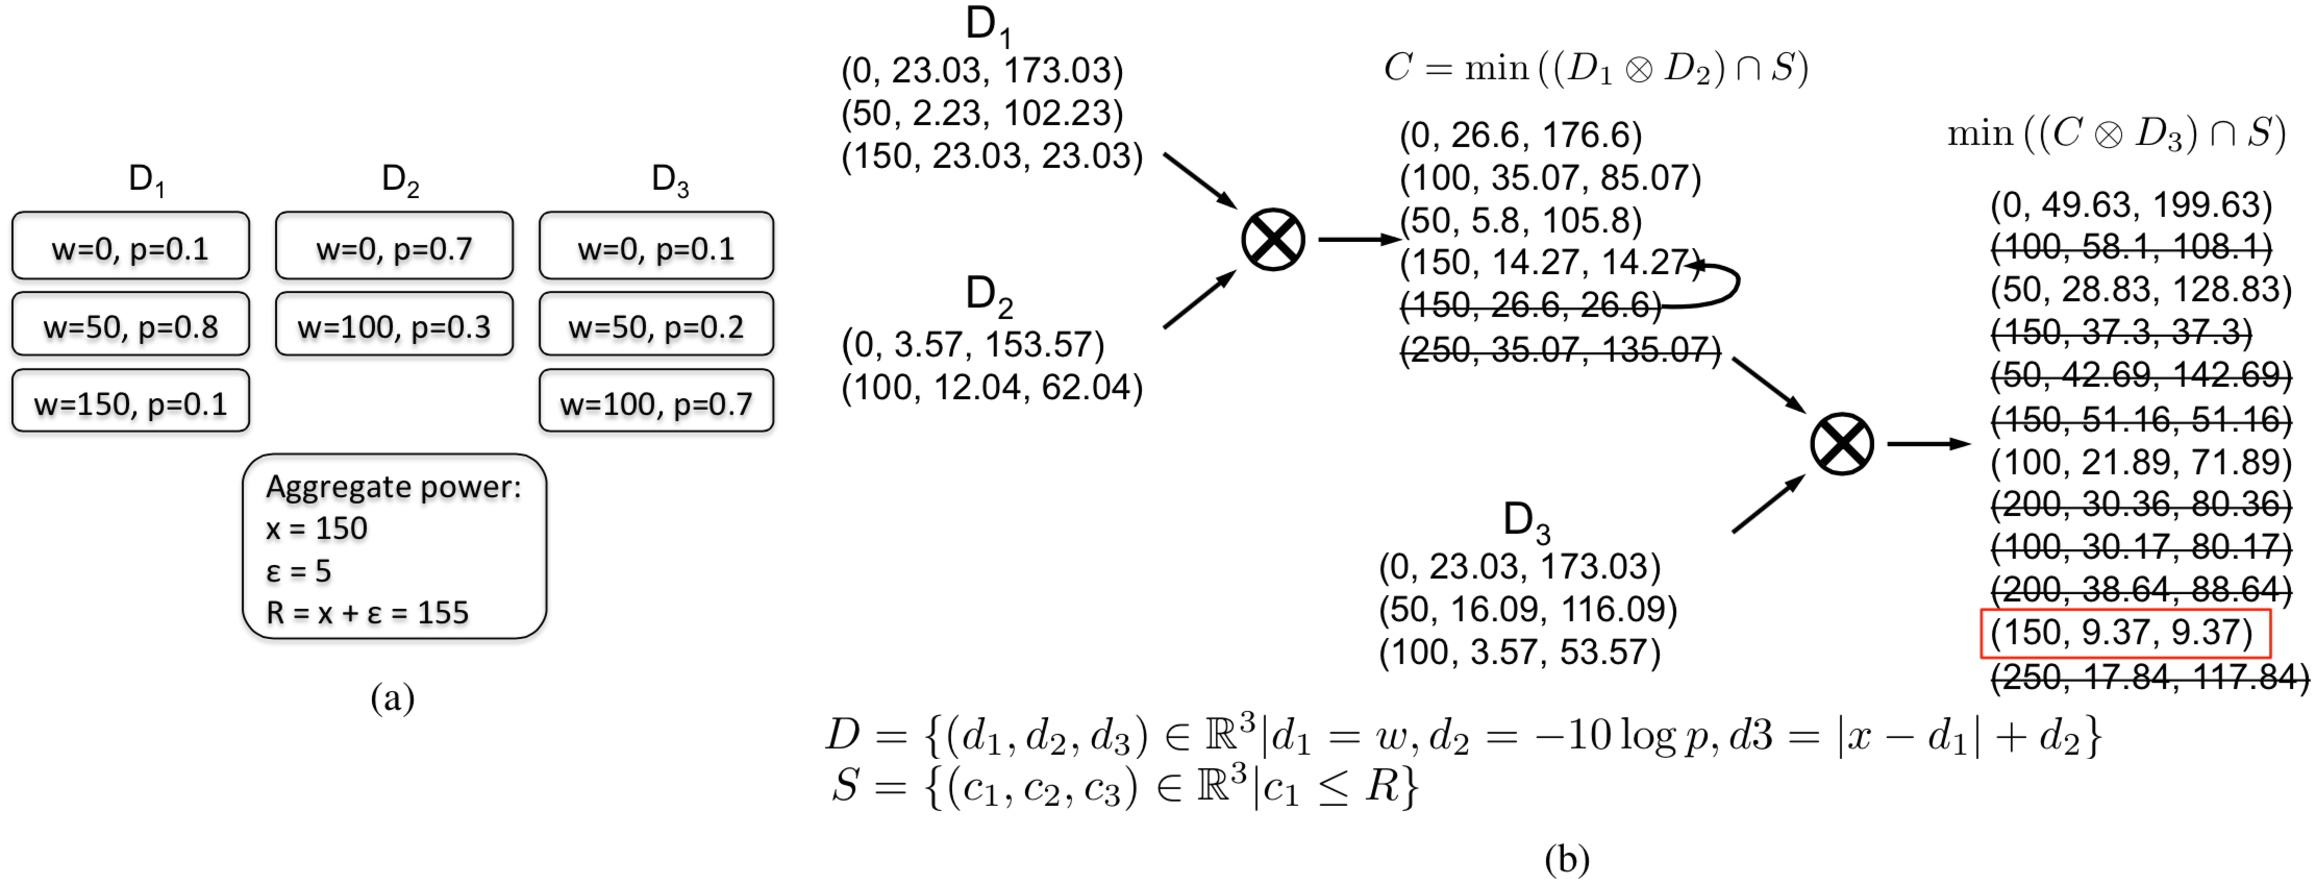
\includegraphics[width=1\textwidth]{./chapters/chapter4/images/CPHex.pdf} 
\caption{Running example of CPH. (a)~Three devices with corresponding power demand and probability of each state as well as the aggregate power consumption. (b)~Each device is represented as a set of tuples, each tuple corresponds to a state. At each iteration, a partial solution can be discarded if its first element (power consumption) exceeds the bound $R$ (rule~1), or its third element is greater than another solution while consuming larger or same power (rule~2). After all sets are combined, the tuple giving the smallest value of the third element is selected as the final solution.} 
\label{fig:SS2} 
\end{figure}

\begin{figure}[ht]
\centering
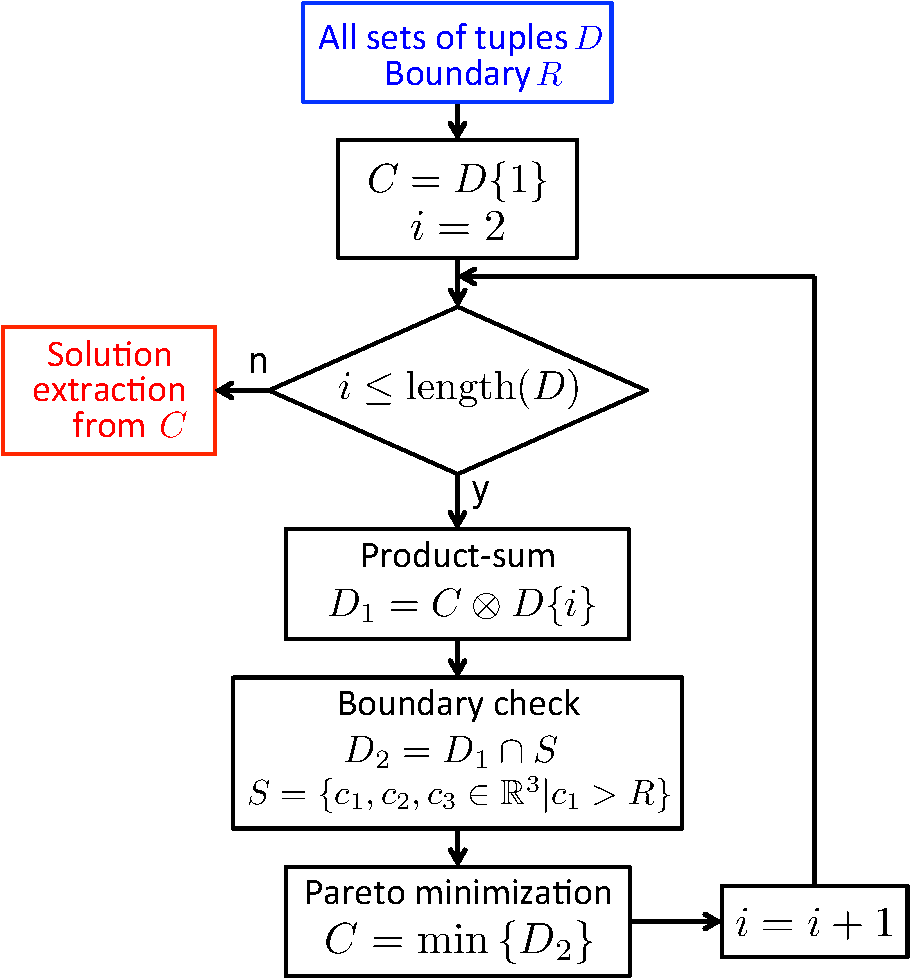
\includegraphics[width=0.55\textwidth]{./chapters/chapter4/images/CPHschema.pdf} 
\caption{CPH algorithm flowchart. All sets of tuples are saved in cell $D$. After the last iteration, the solution is extracted by selecting a tuple in $C$ with the least value of the third dimension.} 
\label{fig:SS2b} 
\end{figure}
In the second step, the sets of tuples are pairwise and iteratively combined by a so-called \textit{product-sum} operation~$\otimes$, which takes all possible combinations from two sets, sums their first and second elements per dimension and then calculates the third element by Eq.~\eqref{eqCPH1}. Some of the partial solutions will be discarded in the third step by two criteria. The first criterion to reject a tuple is that its power demand violates the bound $R$ (rule~1), denoted by the operation $(D_1 \otimes D_2)\cap S$, and the second one is that this tuple is dominated, i.e. it has a greater third value but the same or larger first value than another tuple (rule~2). This process is called \textit{Pareto minimization}~\cite{Shojaei13} and denoted by the operation $C=\min{((D_1 \otimes D_2)\cap S)}$, where $C$ contains the remaining solutions called \textit{Pareto points}. In the final step, after all sets are combined and the Pareto points are found, the point giving the smallest value in the third element is selected as the final solution. 

Figure~\ref{fig:SS2b} resumes the operation of CPH algorithm with
the procedure to combine two sets of tuples presented in Algorithm~\ref{algocph1} and the Pareto minimization illustrated in Algorithm~\ref{algocph2}. The notations $D_1 \preceq D_2$ and $D_1 \prec D_2$ mean that the tuple $D_1$ is dominated and strictly dominated, respectively, by $D_2$.

\begin{algorithm}
\caption{Combine two sets of tuples.} \label{algocph1}
\begin{algorithmic}[1]
\Function{AllComb}{$D_1,D_2,x$}
\State $l1 = \text{length}(D_1)$
\State $l2 = \text{length}(D_2)$
\For {$i=1,\ldots,l1$}
		 \For{$j=1,\ldots,l2$}
		    \State $D\{(i-1)l_1+j\}(1) = D_1\{i\}(1) + D_2\{j\}(1)$
		    \State $D\{(i-1)l_1+j\}(2) = D_1\{i\}(2) + D_2\{j\}(2)$
		    \State $D\{(i-1)l_1+j\}(3) = |D\{(i-1)l_1+j\}(1)-x|+D\{(i-1)l_1+j\}(2)$
		 \EndFor
\EndFor
\State output = $D$
\EndFunction
%\State \textbf{end function}
\end{algorithmic}
\end{algorithm}

\begin{algorithm}
\caption{Pareto minimization.} \label{algocph2}
\begin{algorithmic}[1]
\Function{ParetoMin}{$D,R$}
\State $l = \text{length}(D)$
\State $reject = \text{zeros}(l,1)$
\For {$i=1,\ldots,l$}
    \If {$D\{i\}(1)>R$}
	    \State $reject(i) = 1$
	\EndIf
\EndFor
\State $Ind = \text{find}(reject\neq 1)$
\State $D1 = D\{Ind\}$
\State $l1 = \text{length}(D1)$
\State $reject1 = \text{zeros}(l1,1)$
\For {$i=1,\ldots,l1-1$}
    \For {$j=i+1,\ldots,l1$}
        \If {$reject(j)\neq 1$ and $D1\{i\}\prec D1\{j\}$}
            \State $reject(i)=1$
        \ElsIf {$reject(j)\neq 1$ and $D1\{j\}\preceq D1\{i\}$}
            \State $reject(j)=1$
        \EndIf
    \EndFor
\EndFor
\State $Ind1 = \text{find}(reject1\neq 1)$
\State $D2 = D1\{Ind1\}$
\State output = $D2$
\EndFunction
%\State \textbf{end function}
\end{algorithmic}
\end{algorithm}




\subsubsection{Reed--Solomon codes}\label{DP}
The principle of the DP algorithm to solve the Knapsack problem is that, if the last item is rejected, the best profit will only depend on the remaining items with the full capacity of the knapsack. In contrast, if it is selected, the best profit includes the profit of this item and the best profit obtainable from the remaining items with the remaining capacity of knapsack after subtracting the weight of the last item. 

Therefore, the DP procedure is to construct a profit table with each row corresponding to an item and the number of columns depending on the knapsack capacity with unit step. The profit value of each cell will be calculated based on the current capacity, the corresponding item as well as the recursive relation with the previous cells, which can be explained as follows. At any cell corresponding to an item and a value of capacity, if the item is heavier than the available capacity, it will be rejected and the profit value of the cell is obtained from the previous items. In contrast, it is necessary to compare the profit obtainable with and without that item. The set of the previous items must ensure enough capacity if new item is selected.

\paragraph*{One-state devices}
In the context of one-state devices, each device is considered as an item with its power demand as weight, while the profit is computed from the power demand as well as the operating probability. Although the absolute error between the aggregate power and the total power demand of the identified devices is a criterion to identify the operating devices, it does not satisfy the recursive relation. Concretely,
\begin{eqnarray}
&&\left |\sum_{j=1}^i{w_js_j-x}\right | \neq w_is_i +\left |\sum_{j=1}^{i-1}{w_js_j}-x\right |\\
\mbox{if } &&w_is_i \times \left (\sum_{j=1}^{i-1}{w_js_j}-x\right )<0.\nonumber
\end{eqnarray}

To overcome this restriction, we construct two separated tables, $P^1_e$ and $P^1_l$, for the power and the probability parameters, respectively. Each table is composed of $N$ rows and $R$ columns with $R=\lceil x+\epsilon\rceil$, where $\lceil . \rceil$ is the rounding up operator. The entry of the first table $P^1_e(i,\beta)=\sum_{j=1}^i{w_js_j-x}$ and second table $P^1_l(i,\beta)=\lambda \times \sum_{j=1}^i{L^1(s_j)}$ are calculated by Algorithm~\ref{algo1}. A flag table $F$ is also constructed to mark if a device is running or not.
\begin{algorithm}
\caption{Entry calculation for profit tables in case of one-state devices.}
\label{algo1}
\begin{algorithmic}[1]
\Ensure $P^1_e(i,\beta),P^1_l(i,\beta)$
\State $a^1_1 = P^1_e(i-1,\lfloor \beta-w_i\rfloor)+w_i$
\State $a^1_2 = P^1_l(i-1,\lfloor \beta-w_i\rfloor)+\lambda \times l^1_{i1}$
\State $b^1_1 = P^1_e(i-1,\beta)$
\State $b^1_2 = P^1_l(i-1,\beta)+\lambda \times l^1_{i0}$
\State $A^1 =  \left |a^1_1\right|+a^1_2$
\State $B^1 = \left |b^1_1\right |+b^1_2$
\State $F(i,\beta) = 0$

\If{$w_i \leq \beta$ and $ A^1 \leq B^1$}
  \State $P^1_e(i,\beta) =  a^1_1$
  \State $P^1_l(i,\beta) = a^1_2$
  \State $F(i,\beta) = 1$
\Else
  \State $P^1_e(i,\beta)= b^1_1$
  \State $P^1_l(i,\beta)= b^1_2$
\EndIf
\end{algorithmic}
\end{algorithm}
In Algorithm~\ref{algo1}, because the weight of an item is not an integer number, the notation $\lfloor . \rfloor$ is used to round down the value of $(\beta-w_i)$. The values of $A^1$ and $B^1$ denote the profit obtainable with and without new device in the list of operating ones, respectively. The case that gives better profit is then selected and the respective values are filled in the tables. The initial conditions of each tables are
\begin{eqnarray*}
P^1_e(0,\beta)& =&-x,\beta = 0,\ldots, R\\
P^1_l(0,\beta)& = &0,  \beta = 0,\ldots,R\\
P^1_e(i,0)&=& -x,i=1,\ldots,N\\
P^1_l(i,0) &= &\sum_{j=1}^i{\lambda \times l^1_{j0}},i=1,\ldots,N.
\end{eqnarray*}
After calculating all entries of the profit tables, a backtracking procedure, illustrated in Algorithm~\ref{algo2}, is used to backtrack through the tables from the last cell to obtain the set of running devices with aid of the flag table $F$.

\begin{algorithm}
\caption{Backtracking algorithm in case of one-state devices.}
\label{algo2}
\begin{algorithmic}[1]
\Ensure State indicator vector $\mathbf{s} = \{s_1,\ldots,s_N\}$ 
\State $i = N$
\State $\beta =  R $
\While{$i > 0$ and $\beta>0$}
\If{$P^1_e(i,\beta) \neq P^1_e(i-1,\beta)$ or $F(i,\beta)=1$}
\State $s_i = 1$
\State $\beta = \beta-\lceil w_i \rceil $
\State $i = i-1$
\Else
\State $s_i=0$
\State $i = i-1$
\EndIf
\EndWhile
\end{algorithmic}
\end{algorithm}

Let consider an example for three devices with the respective weight and operating probability: $(w_1,p_1) = (2,0.8)$, $(w_2,p_2) = (5,0.3)$, $(w_3,p_3) = (3.5,0.9)$.
With $P = 10$, $x = 5$, $\epsilon=0.5$, the log-linear form of the operating probability of each device, i.e. $l_{i0} = -\log{(1-p_i)}$ and $l_{i1} = -\log{p_i},i = 1,\ldots,3$, are $(l_{10},l_{11})=(0.7,0.1)$, $(l_{20},l_{21})=(0.15,0.52)$, $(l_{30},l_{31})=(1,0.05)$, respectively, and the boundary of total power $R$ is equal to 6.

The entries of the profit tables are calculated by Algorithm~\ref{algo1} and filled in Table~\ref{table:DP1}. The best profit is obtained at $(i,\beta)=(N,R)$. From this optimal point, the respective combination of running devices can be determined by backtracking through the table by applying Algorithm~\ref{algo2}. As a result, $\mathbf{s} = (1,0,1)$, i.e. the first and third devices are operating while the second one is turned off. Apparently, this combination of devices gives the least absolute error on the power as well as the maximum operating probability.

\begin{table}
\caption{Running example of DP in SmartSense for one-state devices}\label{table:DP1}
\begin{center}
\begin{tabular}{|c|c|c|c|c|c|c|c|}
\hline
\multicolumn{8}{|c|}{$P^1_e(i,\beta)$}\\ \hline 
$(i,\beta)$&0&1&2&3&4&5&6\\ \hline
0&-5&-5&-5&-5&-5&-5&-5 \\ \hline
1&-5&-5&-3&-3&-3&-3&-3 \\ \hline
2&-5&-5&-3&-3&-3&-3&-3 \\ \hline
3&-5&-5&-3&-3&-1.5&-1.5&-0.5 \\ \hline
\multicolumn{8}{|c|}{$P^1_l(i,\beta)$}\\ \hline 
$(i,\beta)$&0&1&2&3&4&5&6\\ \hline
0&0&0&0&0&0&0&0 \\ \hline
1&7&7&1&1&1&1&1\\ \hline
2&8.5&8.5&2.5&2.5&2.5&2.5&2.5\\ \hline
3&18.5&18.5&12.5&12.5&9&9&3\\ \hline
\end{tabular}
\end{center}
\end{table}



\paragraph*{Multi-state devices}

Each multi-state device is considered as a group of items, in which each state is an item with individual weight and profit. Similar to the case of one-state devices, two tables, $P^M_e$ and $P^M_l$, are also constructed to contain the power and probability parameters of the profit. The algorithm to calculate the entries of the first table, $P^M_e(i,\beta)=\sum_{j=1}^i{\sum_{m=1}^{m_i}{(w_{jm}s_{jm}}-x)}$, and the second one, $P^M_l(i,\beta)=P\times \sum_{j=1}^i{L^M(\mathbf{s}_j)},i=1,\ldots,N,\beta=1,\ldots,R$, is detailed in Algorithm~\ref{algo3}. 

\begin{figure}[h]
\centering
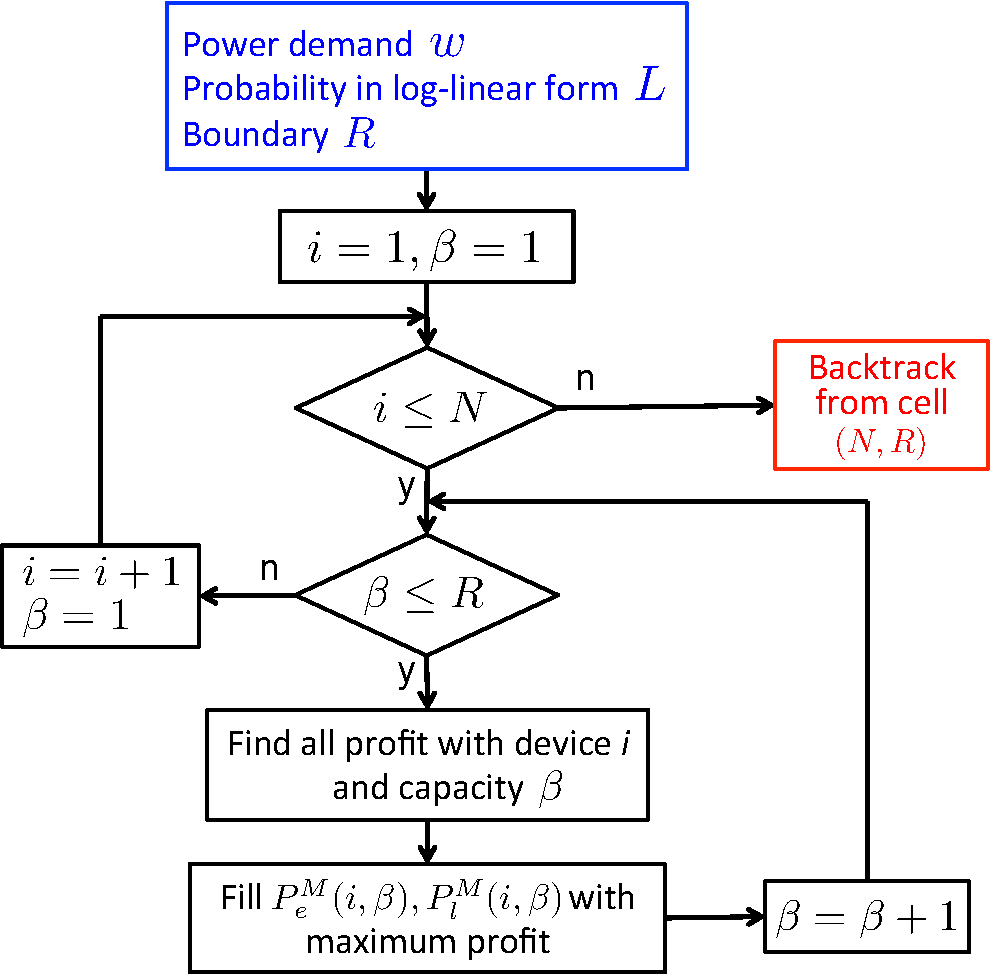
\includegraphics[width=0.6\textwidth]{./chapters/chapter4/images/DPschema.pdf} 
\caption{DP algorithm flowchart. When all entries are filled, the corresponding state vector is obtained by backtracking through the profit tables from the last cell (optimal value).} 
\label{fig:DP1} 
\end{figure}

\begin{algorithm}
\caption{Entry calculation for profit tables in case of multi-state devices.}
\label{algo3}
\begin{algorithmic}[1]
\Ensure $P^M_e(i,\beta),P^M_l(i,\beta)$
\State $Sol(i,\beta) = 0$
\State $a^M_1 = P^M_e(i-1,\beta)$
\State $a^M_2 = P^M_l(i-1,\beta) + \lambda \times l^M_{i0}$
\State $A^M =  \left|a^M_1\right|+a^M_2$
\For{$j=1,\ldots,m_i$}
\If{$w_{ij}\leq \beta$}
\State $b^M_{j1} = P^M_e(i-1,\lfloor \beta-w_{ij}\rfloor)+w_{ij}$
\State $b^M_{j2} = P^M_l(i-1,\lfloor \beta-w_{ij}\rfloor)+\lambda \times l^M_{ij}$
\State $b^M_j = \left|b^M_{j1}\right|+b^M_{j2}$
\Else
\State $b^M_j = +\infty$
\EndIf
\EndFor
\State $k = \min_j{\{b^M_j\}}$; $B^M = b^M_k$
\If{$\min_j{\{w_{ij}\}}\leq \beta$ and $A^M \leq B^M$}
  \State $P^M_e(i,\beta) = a^M_1$
  \State $P^M_l(i,\beta) = a^M_2 $
  \Else
  \State $P^M_e(i,\beta) = b^M_{k1}$
  \State $P^M_l(i,\beta) = b^M_{k2}$
  \State $Sol(i,\beta) = k$
\EndIf
\end{algorithmic}
\end{algorithm}
In other words, the value of each entry when considering a new device is determined by comparing the obtainable profit in two cases: the device is turned off, with profit $A^M$ and the device is operating at a state satisfying the capacity $\beta$, with profit $B^M$.
The initial conditions of the profit tables are
\begin{eqnarray*}
P^M_e(0,\beta) &=& -x,\beta=0,\ldots,R \\
P^M_l(0,\beta)&=&0,\beta = 0,\ldots,R\\
P^M_e(i,0) &=& -x,i=1,\ldots,N\\
P^M_l(i,0)&=&\sum_{j=1}^i{l^M_{j0}},i=1,\ldots,N.
\end{eqnarray*}

To get the state of each device, a backtracking procedure is also constructed as illustrated in Algorithm~\ref{algo4}, in which an additional table $Sol$ with the same size as the profit tables is used to mark the state of devices corresponding to each cell of profit tables.

\begin{algorithm}
\caption{Backtracking algorithm in case of multi-state devices.}
\label{algo4}
\begin{algorithmic}[1]
\Ensure State indicator vector $\mathbf{s} = \{s_1,\ldots,s_N\}$
\State $i = N$ 
\State $\beta =  R$
\While{$i > 0$ and $\beta>0$}
\If{$Sol(i,\beta)>0$}
\State $k = Sol(i,\beta)$
\State $s_i = k$
\State $\beta = \beta-\lceil w_{ik} \rceil $
\State $i = i-1$
\Else
\State $s_i=0$\; $i = i-1$
\EndIf
\EndWhile
\end{algorithmic}
\end{algorithm}

Figure~\ref{fig:DP1} illustrates the flowchart of the proposed DP algorithm in the general case with multi-state devices. Meanwhile, Table~\ref{table:DP2} shows the profit tables relating to the DP algorithm for three multi-state devices with the individual power demand $w_{11}=2$, $(w_{21},w_{22})=(1,4)$, $(w_{31},w_{32}) = (3,5)$ and the respective operating probability $p_{11} = 0.8$, $(p_{21},p_{22}) = (0.7,0.2)$, $(p_{31},p_{32}) = (0.6,0.2)$. The aggregate power consumption $x$ in this example is equal to 6 with standard deviation $\epsilon=0$ and the respective total power boundary $R = \lceil x+\epsilon \rceil = 6$. The regularization parameter $P$ is set to be of $10$. Applying the log-linear form to the operating probability, i.e. $l_{ij} = -\log{p_{ij}},i=1,\ldots,3,j=0,\ldots,m_i$, the corresponding results are $(l_{10},l_{11}) = (0.7,0.1)$, $(l_{20},l_{21},l_{22}) = (1, 0.15, 0.7)$, $(l_{30},l_{31},l_{32}) = (0.7,0.22,0.7)$. Each entry of these tables is calculated by Algorithm~\ref{algo3} and the set of operating state of each device is backtracked through the tables from the optimal point, i.e. $(i,\beta) = (N,R)$, by applying Algorithm~\ref{algo4} is then $\mathbf{s} = (1,1,1)$. This result means that all three devices are operating at the first power state. This determination also satisfies the requirement on the least absolute error on the power consumption and the maximum coincidence operating probability. Presenting vector $\mathbf{s}$ as in Eq.~\ref{eqSS12}, we have $\mathbf{s} = \{1,1,0,1,0\}$.
\begin{table}
\caption{Running example of DP in SmartSense for multi-state devices}\label{table:DP2}
\begin{center}
\begin{tabular}{|c|c|c|c|c|c|c|c|}
\hline
\multicolumn{8}{|c|}{$P^M_e(i,\beta)$}\\ \hline 
$(i,\beta)$&0&1&2&3&4&5&6\\ \hline
0&-6&-6&-6&-6&-6&-6&-6 \\ \hline
1&-6&-6&-4&-4&-4&-4&-4 \\ \hline
2&-6&-5&-5&-3&-3&-3&-3 \\ \hline
3&-6&-5&-5&-3&-3&-3&0 \\ \hline
\multicolumn{8}{|c|}{$P^M_l(i,\beta)$}\\ \hline 
$(i,\beta)$&0&1&2&3&4&5&6\\ \hline
0&0&0&0&0&0&0&0 \\ \hline
1&7&7&1&1&1&1&1\\ \hline
2&17&8.5&8.5&2.5&2.5&2.5&2.5\\ \hline
3&24&15.5&15.5&9.5&9.5&9.5&4.7\\ \hline
\end{tabular}
\end{center}
\end{table}







\section{Energy and power savings from ECC}
The edge detector was firstly proposed in \cite{Hart92} to detect the step-changes on the power signal. Both ED and DTW algorithms at first try to detect the rising edge and falling edge of a device activation and pair them together. Denote $\Delta x(t) = x(t) - x(t-1)$, a rising edge is detected at time $t$ if
$\Delta x(t)\geq \gamma$,
where $\gamma$ is empirically chosen so that it is small enough not to miss the edges, but large enough to ignore the variations in a stable period. In contrast, a falling edge is detected at time $(t-1)$ if $\Delta x(t)\leq -\gamma$. A rising edge and a falling edge are paired together if the difference between their height is lower than a threshold $\alpha$, i.e.,
\begin{equation}
|\Delta x(t_s) - |\Delta x(t_e)||\leq \alpha.
\end{equation}
In the case of multi-state devices, it appears more than one consecutive rising edges or falling edges in an activation. These edges will be grouped together if
\begin{eqnarray}
\left|\sum_{i=1}^{n_s}{\Delta x(t_s^i)}-\left |\sum_{i=1}^{n_e}{\Delta x(t_e^i)}\right| \right|\leq \alpha,
\end{eqnarray}
where $n_s$, $n_e$ are the number of consecutive rising edges and falling edges, respectively.

In the ED algorithm, a feature is composed of the first rising edge and the last falling edge, while all active power values between them are used in DTW feature. To improve the performance of the edge detector, a median filter can also be applied to remove the peaks~\cite{Norford96,Marceau2000ECM}.

\subsection{Results}
In training period, all possible patterns of each device are extracted and saved in the library $\mathbf{EDlib}$, in which pattern $j$ of device $i$ is denoted as 
\begin{equation}
f_{ij}^{ed} = \{\Delta x_{ij}^R,\Delta x_{ij}^F\},
\end{equation}
with notation $R$ for rising edge and $F$ for falling edge.
If the edge detector detects an event switched on at time $t_s$ and switched off at time $t_e$, the corresponding feature is
\begin{equation}
f^{ed} = \{\Delta x(t_s^1),\Delta x(t_e^{n_e})\}.
\end{equation}
The distance between two patterns $f_{ij}^{ed}$ and $f^{ed}$ can be calculated as
\begin{eqnarray}\label{eqED1}
\delta_{ij}^{ed} &=& d(f^{ed},f_{ij}^{ed})\nonumber \\
&=&|\Delta x(t_s^1)-\Delta x_{ij}^R|+|\Delta x(t_e^{n_e})-\Delta x_{ij}^F|.
\end{eqnarray}
In the ED algorithm, the detected event will be matched with the device having a pattern with the minimum distance. Nevertheless, in homes and buildings, there are several devices with the same edge height, which decreases the load disaggregation performance. To overcome this challenge, in SmartSense, the probability that each device $i, i=1,\ldots,N$, is turned on and off at the same time as the detected event, denoted as $p_i^R(t_s^1)$ and $p_i^F(t_e^{n_e})$, respectively, is estimated as in Section~\ref{model}. This means, $p_i^R(t_s^1)=(1-npv)$ if a rising edge of device $i$ is detected at time $t_s^1$ and $p_i^R(t_s^1)=(1-npv)$ on the contrary. Similarly, $p_i^F(t_e^{n_e})=pr$ if device $i$ has a falling edge at time $t_e^{n_e}$ and $p_i^F(t_e^{n_e})=(1-npv)$ on the contrary. In the case of unsupervised devices, $p_i^R(t_s^1) = p_i^F(t_e^{n_e}) = 0.5$. The coincidence probability that both edges appear is then
\begin{equation}\label{eqED2}
Pr_i^{ed} = p_i^R(t_s^1)\times p_i^F(t_e^{n_e}).
\end{equation}

To reduce the computational complexity, the multiplication in Eq.~\eqref{eqED2} can be transformed to an addition by applying the log-linear form, which gives
\begin{eqnarray}\label{eqED3}
\phi_i^{ed} &=& -\log{Pr_i^{ed}}\nonumber \\
&=& -\log{p_i^R(t_s^1)}-\log{p_i^F(t_e^{n_e})}.
\end{eqnarray}
The identified device does not only have a pattern with the minimum distance $\delta_{ij}^{ed}$, but also has the maximum probability $Pr_i^{ed}$, i.e. the minimum log-linear form $\phi_i^{ed}$. In other words, the ED algorithm will try to find the pattern giving the minimum modified distance, calculated as
\begin{eqnarray}
d_{ij}^{ed} = \delta_{ij}^{ed}+\lambda_1\times \phi_i^{ed},
\end{eqnarray}
where $\lambda_1$ is a regularization parameter. The load identification procedure for each detected pattern is presented in Algorithm~\ref{algo:ED1}, where $\Phi^{ed}$ contains the probability in log-linear form of all devices and $m_i$ denotes the number of patterns of device $i$ in $\mathbf{EDlib}$. The procedure is illustrated by a flowchart in Figure~\ref{fig:ed1}.
\begin{figure}[!h]
\centering
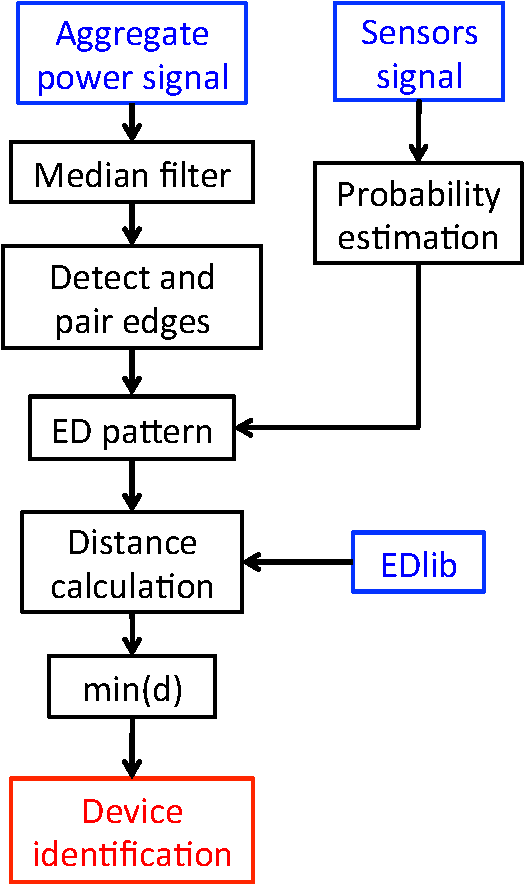
\includegraphics[width=0.45\textwidth]{./chapters/chapter4/images/EDschema.pdf} 
\caption{Load disaggregation based on the ED algorithm.} 
\label{fig:ed1} 
\end{figure}

\begin{algorithm}
\caption{Matching detected event in ED.}\label{algo:ED1}
\begin{algorithmic}[1]
\Function{EDiden}{$f^{ed},\Phi^{ed},\mathbf{EDlib}$}
\State $MIN = +\infty$
\State $k = 0$
	\For {$i=1,\ldots,N$}
	    \State{$\phi^{ed}_i=\Phi^{ed}(i)$}
		 \For{$j=1,\ldots,m_i$}
		    \State $f_{ij}^{ed} = \mathbf{EDlib}\{i,j\}$
		    \State $\delta_{ij}^{ed} = |\Delta x(t_s^1)-\Delta x_{ij}^R|+|\Delta x(t_e^{n_e})-\Delta x_{ij}^F|$
		    \State $d_{ij}^{ed} = \delta_{ij}^{ed}+\lambda_1\times \phi_i^{ed}$
		    \If{$d_{ij}^{ed}\leq MIN$}
		        \State $MIN = d_{ij}^{ed}$
		        \State $k = i$
		    \EndIf
		 \EndFor
	\EndFor
	%\State \textbf{end for}
\State output = $k$
\EndFunction
%\State \textbf{end function}
\end{algorithmic}
\end{algorithm}



\subsection{Analyzing}
Different from the ED algorithm, in DTW, all active power values between the first rising edge and the last falling edge are extracted to comprise a pattern, i.e. $f^{dtw}=\{f^{dtw}(k)|k=1,\dots,t_e^{n_e}-t_s^1+1\}$, which
\begin{eqnarray}
f^{dtw}(k)=\begin{cases}
h_s^i, & z_s^i\leq k <z_s^{i+1},1\leq i \leq n_s-1\\
h_s^{n_s}+\frac{h_e^1-h_s^{n_s}}{z_e^1-z_s^{n_s}}\left(k-z_s^{n_s} \right), & z_s^{n_s}\leq k \leq z_e^1\\
h_s^{i+1}, & z_e^i < k \leq z_e^{i+1},1< i\leq n_e-1
\end{cases}
\end{eqnarray}
where $h_s^i = \sum_{j=1}^i{\Delta x(t_s^j)}$, $h_e^i=\left|\sum_{j=i}^{n_e}{\Delta x(t_e^j)}\right|$, $z_s^i=t_s^i-t_s^1+1$, and $z_e^i=t_e^i-t_s^1+1$.
Figure~\ref{fig:dtw2} illustrates a DTW pattern with two rising edges and two falling edges.
\begin{figure}[!h]
\centering
\centerline{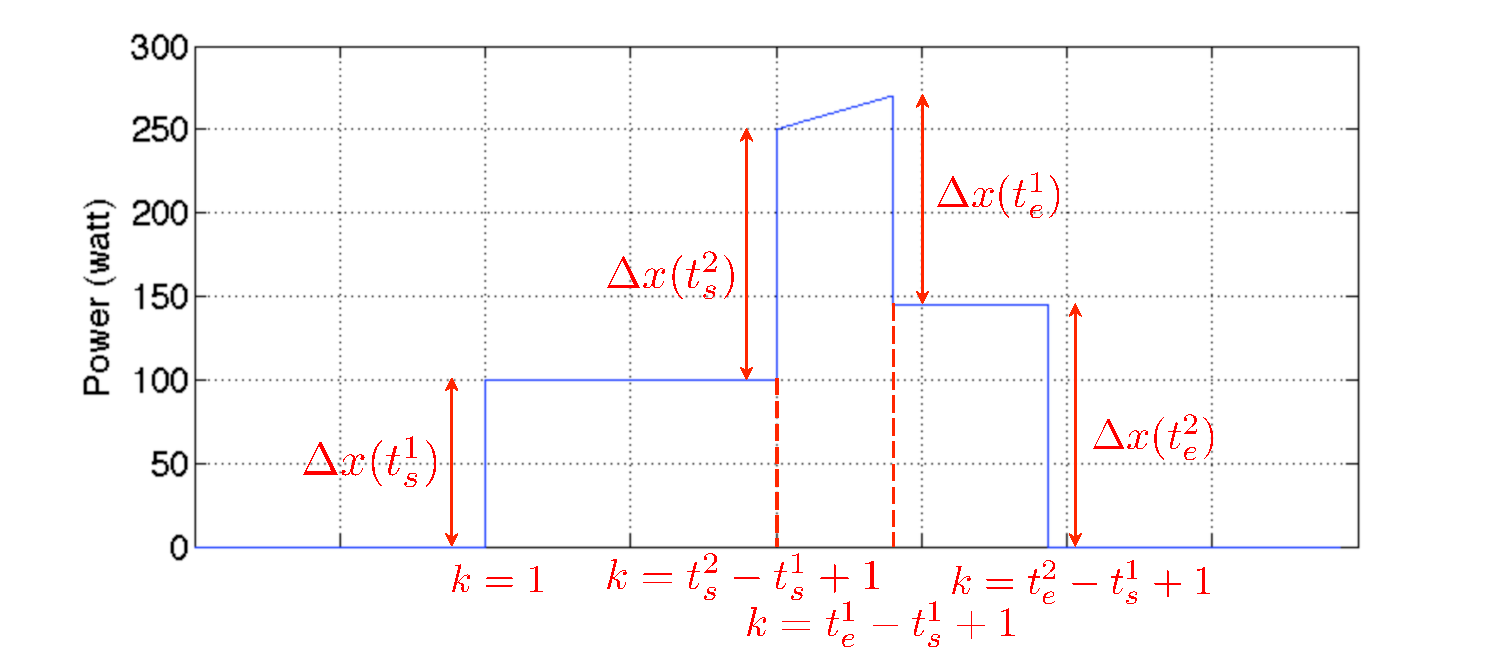
\includegraphics[width=0.8\textwidth]{./chapters/chapter4/images/dtwpattern.pdf}}
\caption{DTW pattern.}
\label{fig:dtw2}
%
\end{figure}
All possible patterns of each device are extracted and saved in library $\mathbf{DTWlib}$ from the training period. Because the length of patterns is different, the accumulated distance between the detected pattern $f^{dtw}$ and a pattern $j$ of device $i$ in the library is calculated by Algorithm~\ref{algo:DTW1}. Concretely,
\begin{equation}\label{eqDTW1}
\delta_{ij}^{dtw} = AccDistance(f^{dtw},f_{ij}^{dtw}).
\end{equation}
\begin{algorithm}
\caption{Accumulated distance between two different length vectors~\cite{Liao14}.} \label{algo:DTW1}
\begin{algorithmic}[1]
\Function{AccDistance}{$f1,f2$}
\State $l1 = \text{length}(f1)$
\State $l2 = \text{length}(f2)$
\State $\delta(0,0) = 0;\delta(i,0) = \delta(0,i) = +\infty$
	\For {$i=1,\ldots,l1$}
		 \For{$j=1,\ldots,l2$}
		    \State $d(i,j) = |f1(i)-f2(j)|$
		    \State $\delta(i,j) = d(i,j)+\min{\{\delta(i-1,j),\delta(i-1,j-1),\delta(i,j-1)\}}$
		 \EndFor
	\EndFor
	%\State \textbf{end for}
\State output = $\delta(l1,l2)$
\EndFunction
%\State \textbf{end function}
\end{algorithmic}
\end{algorithm}

In~\cite{Liao14}, the detected pattern will be matched to the device having a pattern with minimum accumulated distance calculated by Eq.~\eqref{eqDTW1}. 
However, in SmartSense, in order to improve the performance, the operating probability of each device during the same period as the detected event will also be used in log-linear form, and is defined as
\begin{eqnarray}
Pr_i^{dtw} &=& \prod_{t=t_s^1}^{t_e^{n_e}}{p_i(t)}\\
\phi_i^{dtw} &=& -\log{Pr_i^{dtw}}\nonumber \\
&=& -\sum_{t=t_s^1}^{t_e^{n_e}}{\log{p_i(t)}},\label{eqDTW2}
\end{eqnarray}
where $p_i(t)$ is the on-state probability of device $i$ at time instant $t$, estimated as in Section~\ref{model}, i.e. $p_i(t) =pr$ if device $i$ is detected as on and $p_i(t) = (1-npv)$ if detected as off. In the case of unsupervised devices, $p_i(t) = 0.5$. The load identification, as presented in Algorithm~\ref{algo:DTW2}, is not only based on the accumulated distance as in Eq.~\eqref{eqDTW1}, but also considers the operating probability of each device in Eq.~\eqref{eqDTW2}. The probability in log-linear form of all devices is contained in vector $\Phi^{dtw}$. A modified distance then combines these two parameters with a regularization parameter $\lambda_2$, which gives
\begin{equation}
d_{ij}^{dtw} = \delta_{ij}^{dtw} + \lambda_s\times \phi_i^{dtw}.
\end{equation}
The pattern giving the minimum distance will be selected to identify the corresponding device. Because the length of patterns strongly affects the accumulated distance, the DTW algorithm is only suitable for devices with fixed on-duration, such as fridge, washing machine, dish washer. Other devices controlled by the human intervention, e.g. lamp, computer, etc., cannot be exactly identified. Therefore, we propose to combine DTW with ED, in which $\mathbf{DTWlib}$ only contains the patterns of fixed on-duration devices and $\mathbf{EDlib}$ saves the edge patterns of the others. The flowchart of the proposed DTW algorithm is shown in Figure~\ref{fig:dtw1}. A threshold $\beta$ is used to reject a DTW pattern if it does not match with any one in $\mathbf{DTWlib}$. The detected pattern will be then extracted based only on the first rising edge and the last falling edge, by applying the ED procedure.
\begin{algorithm}
\caption{Matching detected event in DTW.}\label{algo:DTW2}
\begin{algorithmic}[1]
\Function{DTWiden}{$f^{dtw},\Phi^{dtw},\mathbf{DTWlib}$}
\State $MIN = +\infty$
\State $k = 0$
	\For {$i=1,\ldots,N$}
	    \State{$\phi_i^{dtw}=\Phi^{dtw}(i)$}
		 \For{$j=1,\ldots,m_i$}
		    \State $f_{ij}^{dtw} = \mathbf{DTWlib}\{i,j\}$
		    \State $\delta_{ij}^{dtw} = AccDistance(f^{dtw},f_{ij}^{dtw})$
		    \State $d_{ij}^{dtw} = \delta_{ij}^{dtw} + \lambda_2\times \phi_i^{dtw}$
		    \If{$d_{ij}^{dtw}\leq \beta$ and $d_{ij}^{dtw}\leq MIN$}
		        \State $MIN = d_{ij}^{dtw}$
		        \State $k = i$
		    \EndIf
		 \EndFor
	\EndFor
	%\State \textbf{end for}
\State output = $k$
\EndFunction
%\State \textbf{end function}
\end{algorithmic}
\end{algorithm}

\begin{figure}[!ht]
\centering
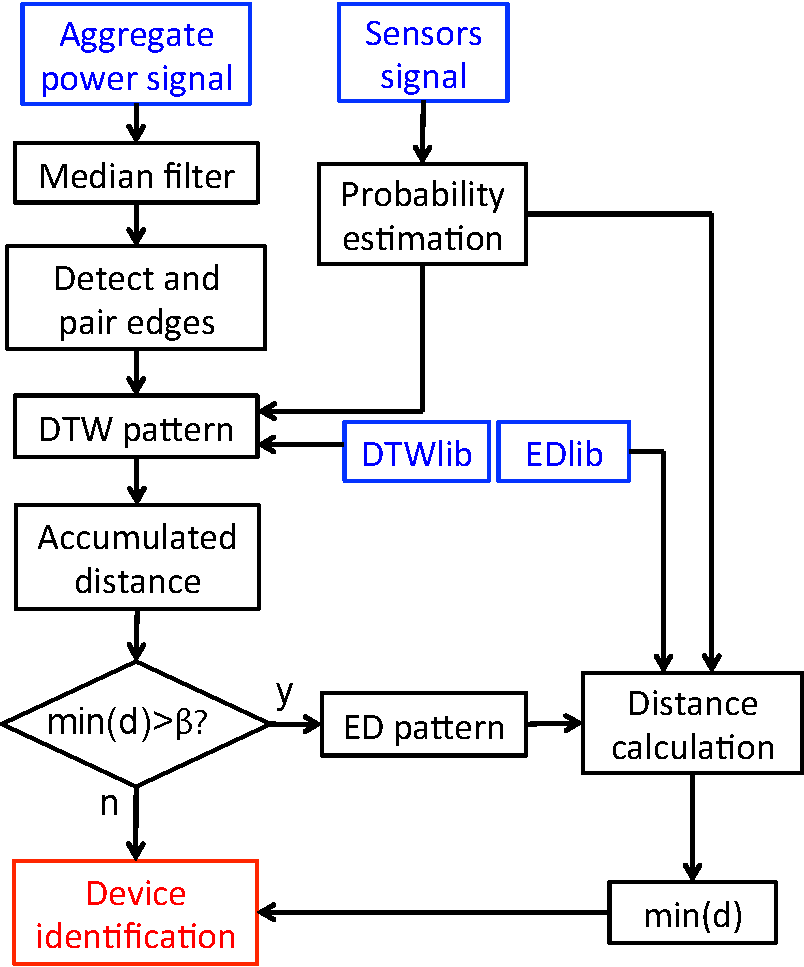
\includegraphics[width=0.65\textwidth]{./chapters/chapter4/images/DTWschema.pdf} 
\caption{Combination of DTW and ED algorithms. A threshold $\beta$ is used to reject a pattern if it does not match with any one in $\mathbf{DTWlib}$} 
\label{fig:dtw1} 
\end{figure}


\section{Conclusion}

